\documentclass[a4paper]{article}


\usepackage[pdftex,pdfauthor={Shabaz Sultan},pdftitle={Colloquium Report 1},colorlinks=true, linkcolor=black,          % color of internal links
    citecolor=black,        % color of links to bibliography
    filecolor=black,      % color of file links
    urlcolor=black   ]{hyperref}
\usepackage[pdftex]{graphicx}
\usepackage{amsmath}
\usepackage{float}

\author{Chi Chun Wan - 2525244\\
Shabaz Sultan - 2566703\\
Boudewijn Zwaal - 1897527}
\title{Heuristics, Algorithm Flowcharts team CSB}
\begin{document}
\maketitle
\section{Flowcharts}
We made flowcharts for the two algorithms we've used to find the best tour, namely hill-climbing and Simulated Annealing.
\subsection{Hill Climbing}
\begin{figure}[H]
    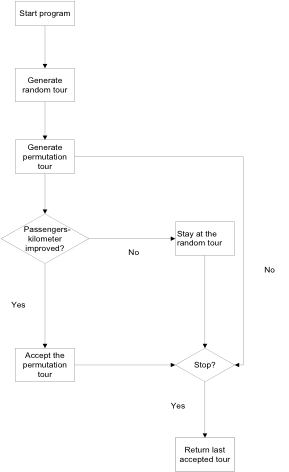
\includegraphics[scale=0.7]{hillclimb_chart.png}
\end{figure}
In case of hill-climbing, we start with an initial random tour. To find a better solution, we permutate the tour by randomly selecting a sub-tour in the initial tour and replace it with another possible valid sub-tour. Care is taken to not remove the homebase airport from the tour. The score of the passenger-kilometers for the initial tour is stored in a variable best score. If the score of the permutation tour is higher than the score of the arbitrary tour, the score of the permutated tour will be the new best score and the permutation tour will be accepted, otherwise the best score will stay the same and we will stay at the previous tour. This process is repeated until no further improvements can be found and the best tour is the last accepted tour. \\
When applied to multiple planes, first one of the planes in the system is randomly chosen and its flightplan (tour) is permutated. The total score of all airplane tours is then calculated and compared to the previous best score. If it improves on said score, the new tour is accepted.

\subsection{Simulated Annealing}
\begin{figure}[H]
    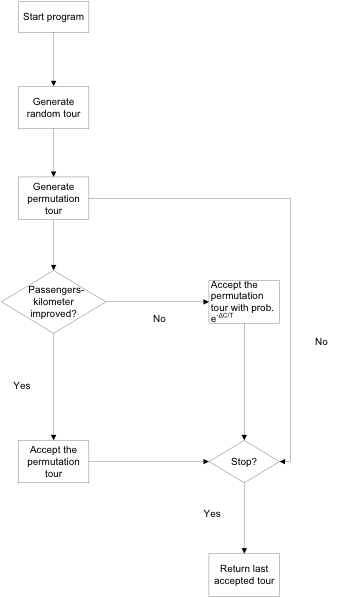
\includegraphics[scale=0.6]{sa_chart.png}
\end{figure}
In case of simulated annealing, it's almost the same as hill climbing except when the passengers-kilometer score is not improved, you will accept the permutation tour with probability $P=e^{\frac{-\Delta C}{T}}$, where $\Delta C= \text{score of the permutation tour}-\text{score of the current best tour}$ and $T=0,999^i*T_0$ with i is the number of iterations and $T_0$  is the start temperature 50.000.
This probability will decrease with the number of iterations. Thus when the number of iterations increases, the temperature goes down. When temperature is high, the system will choose new states more or less at random, but as the temperature lowers this algorithm will go to hill-climbing. 

\end{document}

